\documentclass[10pt]{beamer}
\usetheme[outer/progressbar=foot]{metropolis}
\usepackage{booktabs}
%\usepackage[scale=2]{ccicons}
\usepackage{pgfplots}
\usepackage{cancel}
\usepackage[ngerman]{babel}
\usepackage[utf8]{inputenc}
\usepackage{blindtext}
\usepackage{amsmath}
\usepackage[italicdiff]{physics}
\usepackage[italic]{hepnames}
\usepackage{graphicx}
\usepackage{float}
\usepackage{color}
\usepackage{physics}
\usepackage{tikz}
\usepackage[absolute,overlay]{textpos}
\usepackage[texcoord,grid,gridcolor=red!10,subgridcolor=green!10,gridunit=pt]{eso-pic}

\usepgfplotslibrary{dateplot}


%Frontpage
\title{Calorimetry and Deep Learning}
\date{\today}
\author{Simon Schnake}
\institute{Universität Hamburg}

%Document
\begin{document}
\maketitle
\tikzstyle{every picture}+=[remember picture]
\begin{frame}{Calorimetry in Particle Physics}

\end{frame}

\begin{frame}{Deep Learning}

\end{frame}

\begin{frame}{Simulation Setup}
  \begin{columns}
    \column{0.5\textwidth}
    \begin{textblock*}{150pt}(2pt,55pt)
      \begin{itemize}
      \item Simulation with Geant4\small{}
      \item $e^-$ from 0. to 10 GeV
      \item 300,000 events
      \end{itemize}
    \end{textblock*}
    \begin{textblock*}{10pt}(2pt,125pt)
      \begin{tabular}{l|l|l}
        layer  & scint    & absorber \\ \hline
        layer 0      & 9mm     & 40 mm SS\\
        layer 1 - 8  & 3.7mm   & 50.5 mm brass        \\
        layer 9 - 14 & 3.7mm   & 56.5 mm brass         \\
        layer 15     & 3.7 mm  & 75 mm SS \\
        layer 16     & 9mm     &                      
      \end{tabular}
    \end{textblock*}
    \column{0.5\textwidth}
    \begin{figure}[htp]
      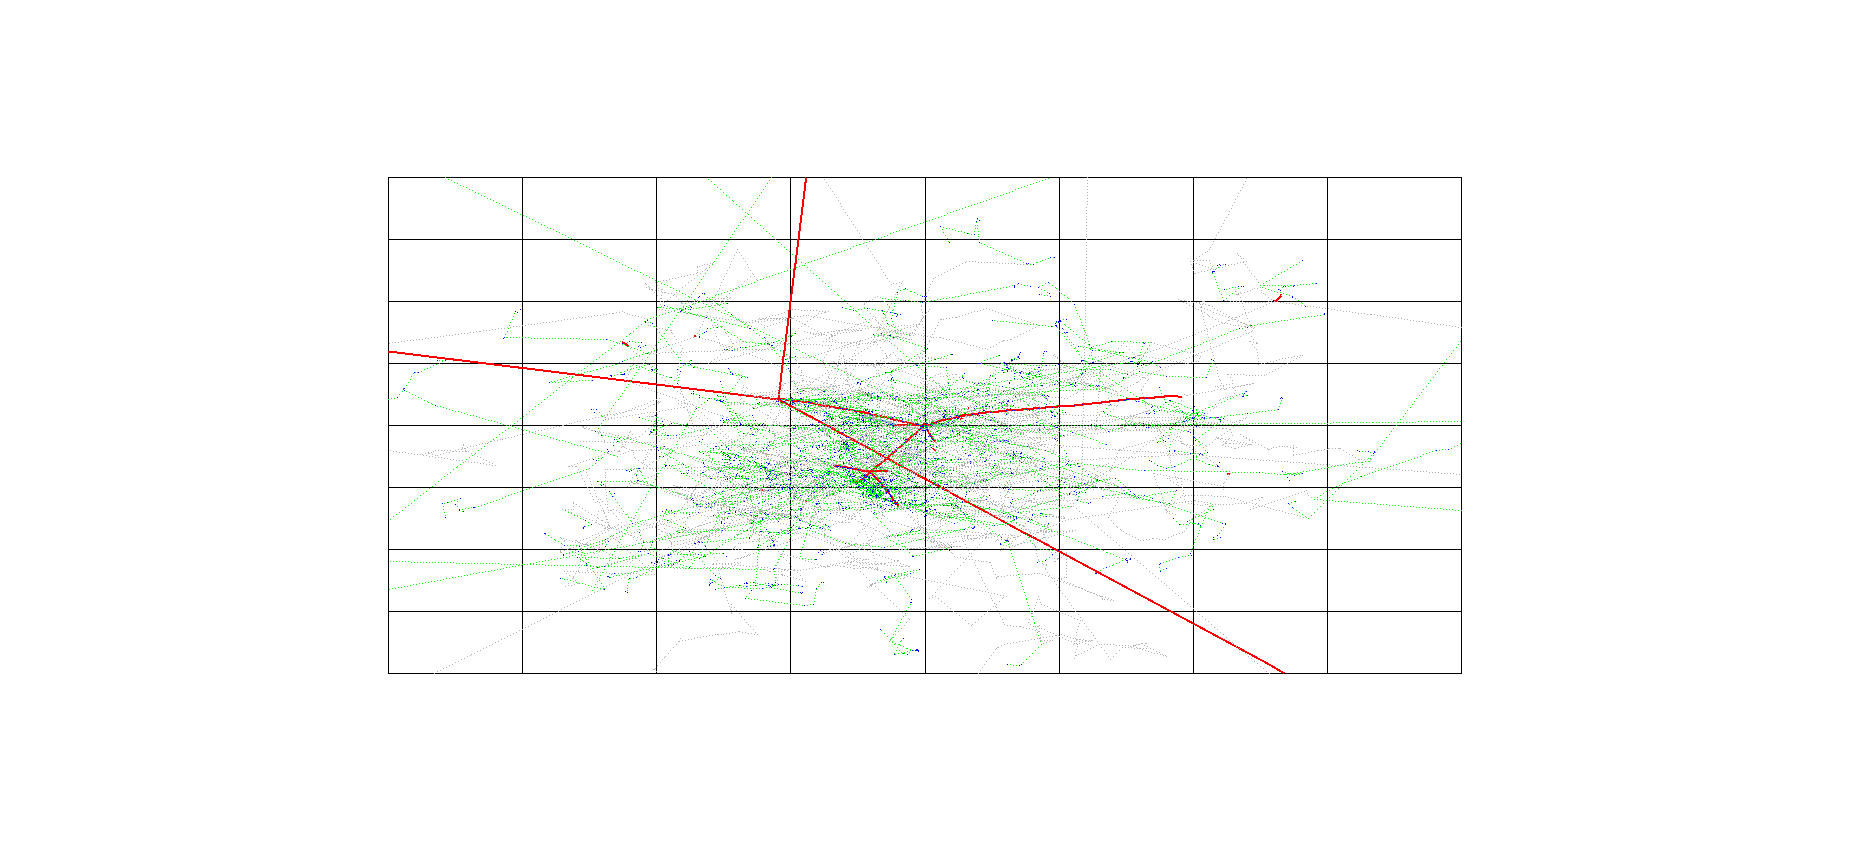
\includegraphics[width=1.1\textwidth]{front.png}\\
      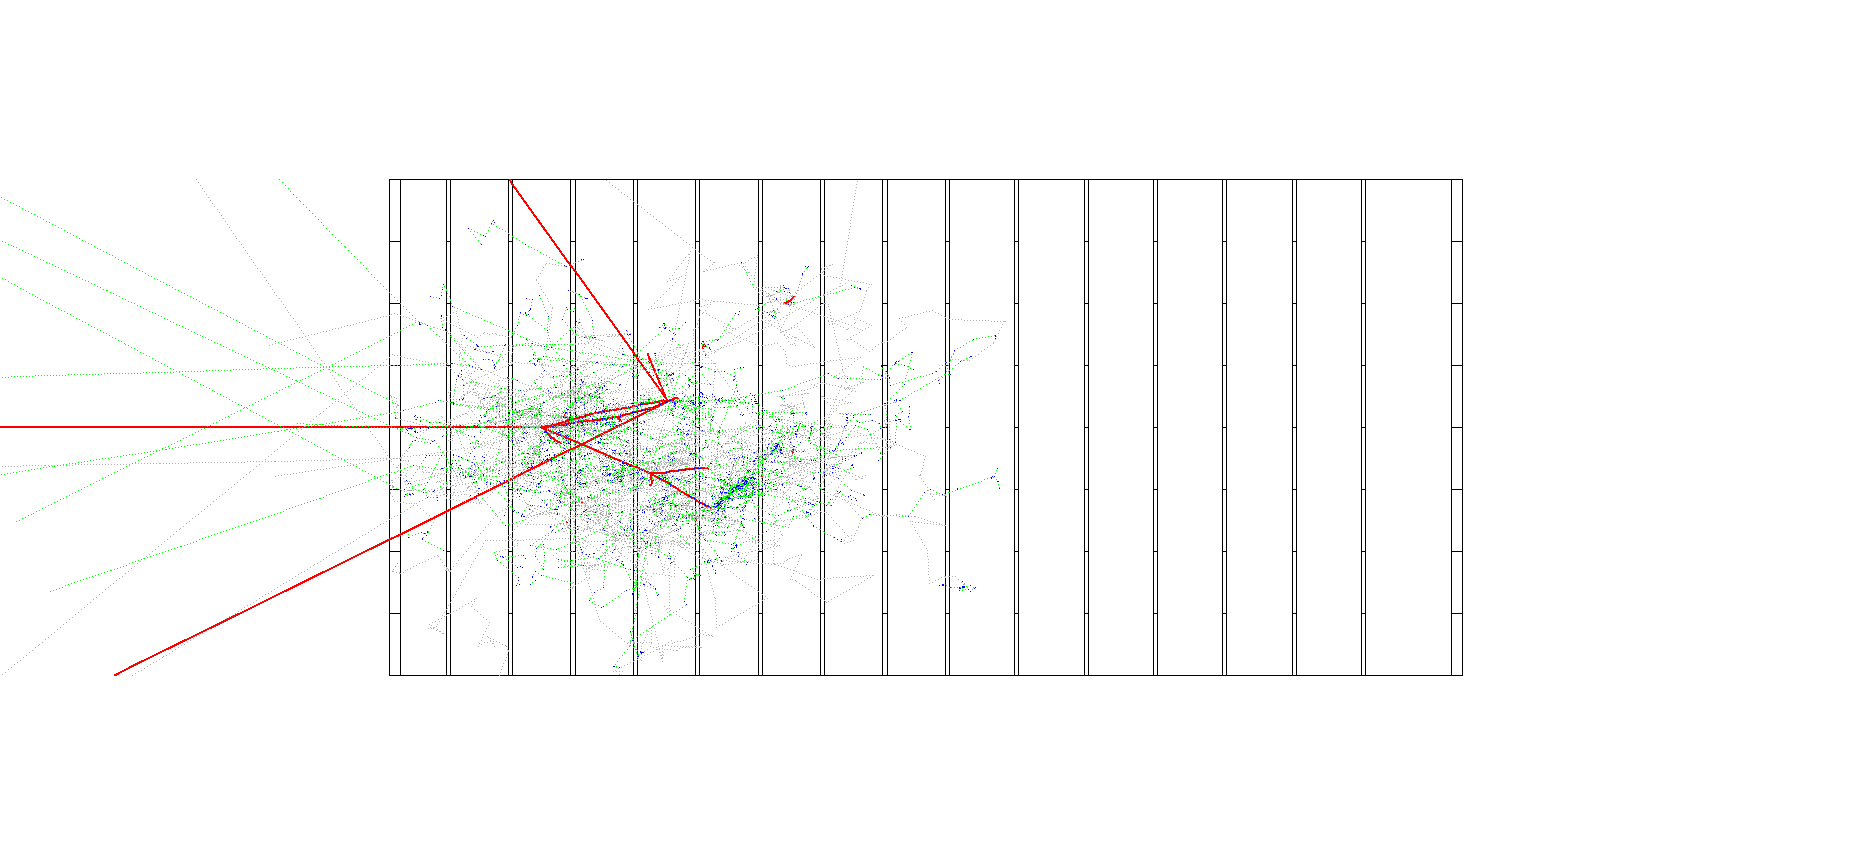
\includegraphics[width=1.1\textwidth]{side.png}
    \end{figure}
  \end{columns}
  \begin{textblock*}{100pt}(250pt,70pt)
    Front view
  \end{textblock*}
  \begin{textblock*}{100pt}(250pt,150pt)
    Side view
  \end{textblock*}
\end{frame}

\begin{frame}{Resulting Data}
  \begin{columns}
    \column{0.5\textwidth}
    \begin{figure}[htp]
      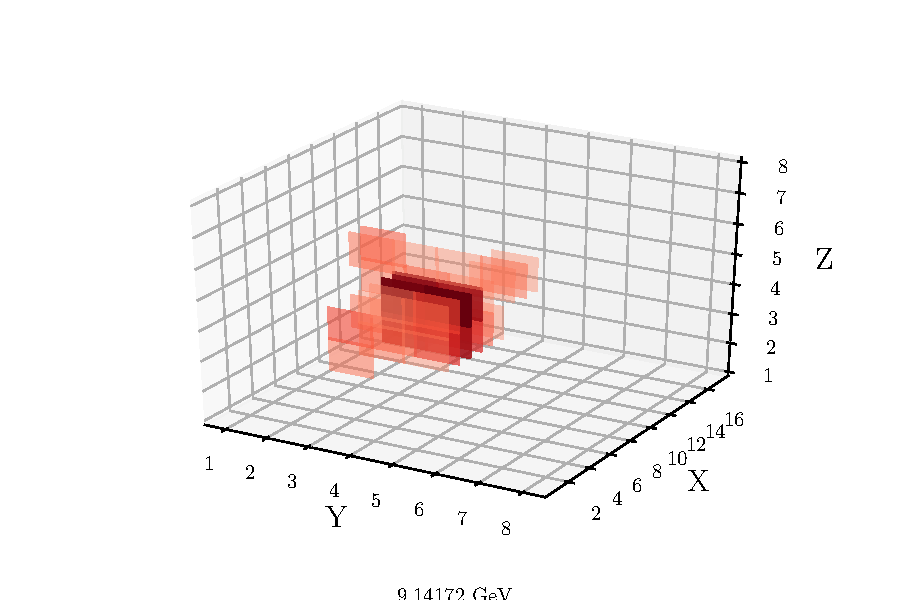
\includegraphics[width=1.1\textwidth]{../data_display.pdf}
    \end{figure}
    \column{0.5\textwidth}
    \begin{figure}[htp]
      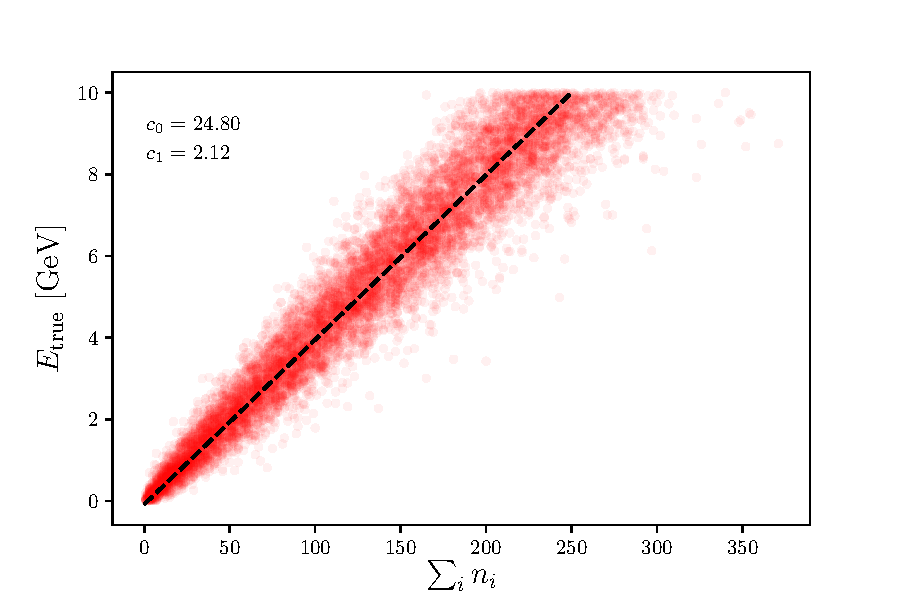
\includegraphics[width=\textwidth]{../e-vs-sum_n_fit.pdf}
    \end{figure}
  \end{columns}
\end{frame}

\begin{frame}{Neuralnet}
  \begin{itemize*}
  \item 
    \begin{tabular}{l|l|l}
      Layer & Type                                & Activation \\ \hline
      1     & Conv2D(32, (2,2), strides = (1, 1)) & ReLu       \\
      2     & Flatten()                           &            \\
      3-5   & Dense(128)                          & ReLu       \\
      6     & Dense(10)                           & ReLu       \\
      7     & Dense(1)                            & Linear    
    \end{tabular}
  \item Loss = Mean Squared Error
  \item Optimizer = Rmsprop
  \end{itemize*}
\end{frame}

\begin{frame}{First Results of the Neuralnet}
  \begin{columns}
    \column{0.5\textwidth}
    \begin{figure}[htp]
      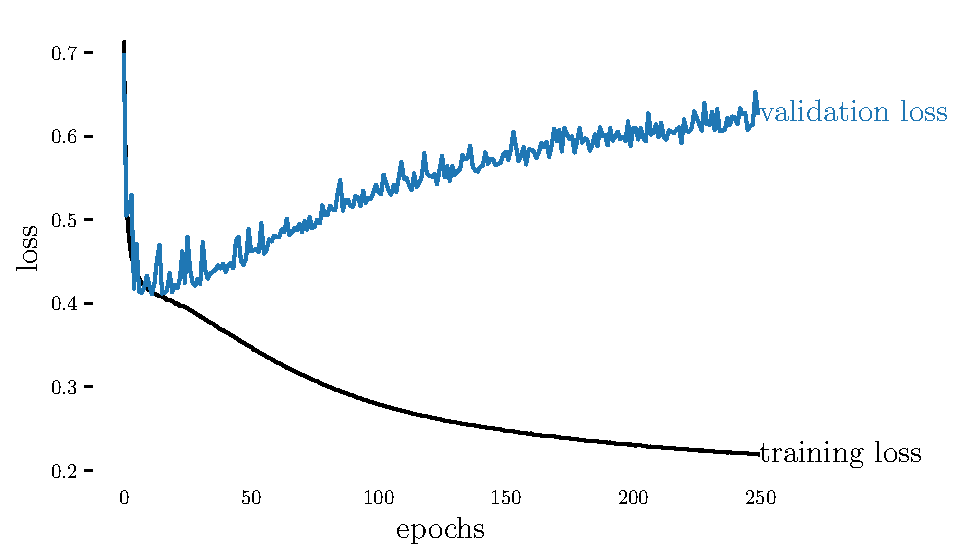
\includegraphics[width=1.1\textwidth]{../first_loss.pdf}
    \end{figure}
    \column{0.5\textwidth}
    \begin{figure}[htp]
      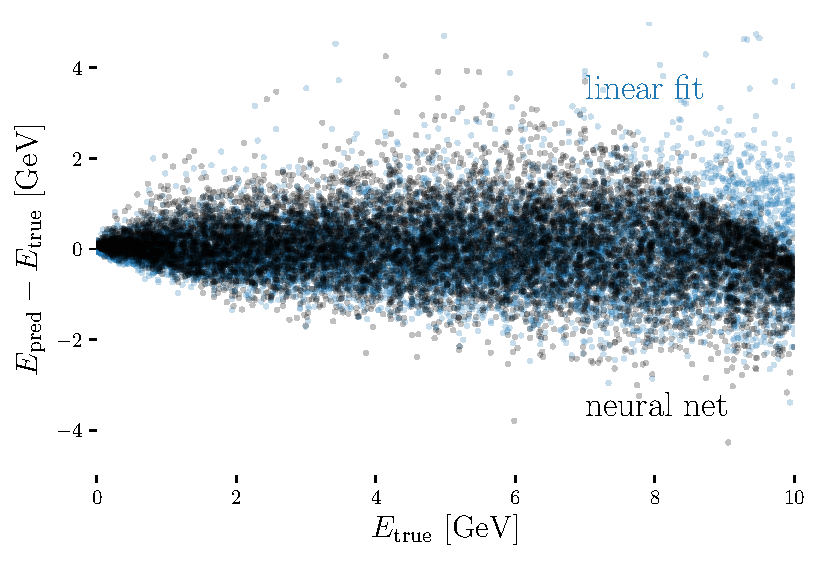
\includegraphics[width=1.1\textwidth]{../first.pdf}
    \end{figure}
  \end{columns}
\end{frame}

\begin{frame}{Data Augmentation}
  \begin{itemize}
  \item flip the data arrays in the y axes
  \item rotate around the x axes
  \item shift in y and z
  \end{itemize}
    \begin{figure}[htp]
      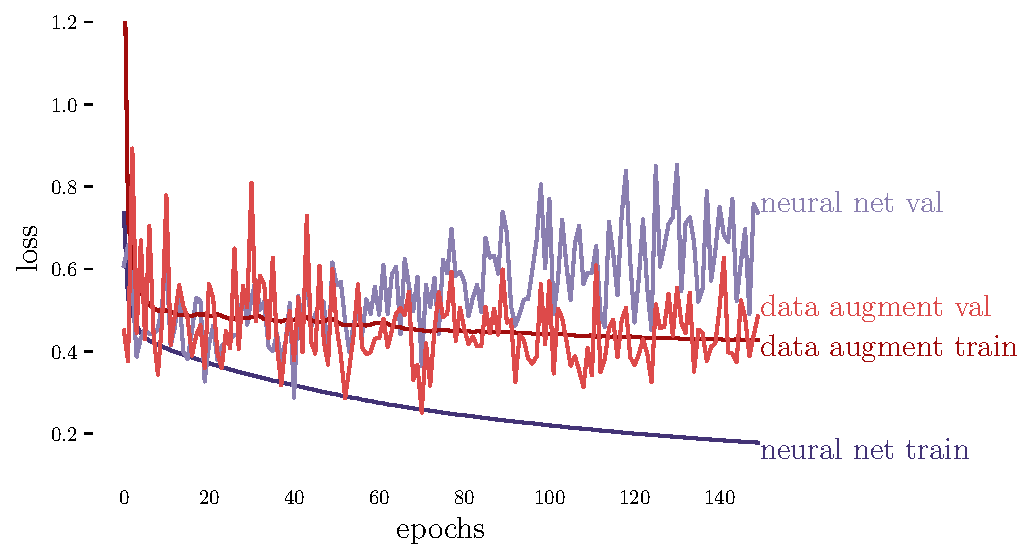
\includegraphics[width=0.8\textwidth]{../data_augment_loss.pdf}
    \end{figure}
\end{frame}


\begin{frame}{Data Augmentation}
  \begin{columns}
    \column{0.5\textwidth}
    \begin{figure}[htp]
      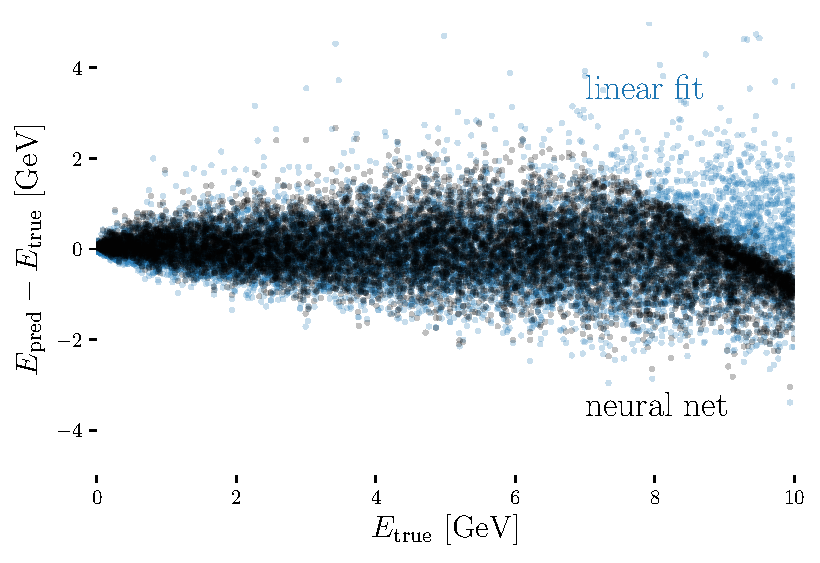
\includegraphics[width=1.1\textwidth]{../data_augment.pdf}
    \end{figure}
    \column{0.5\textwidth}
    \begin{figure}[htp]
      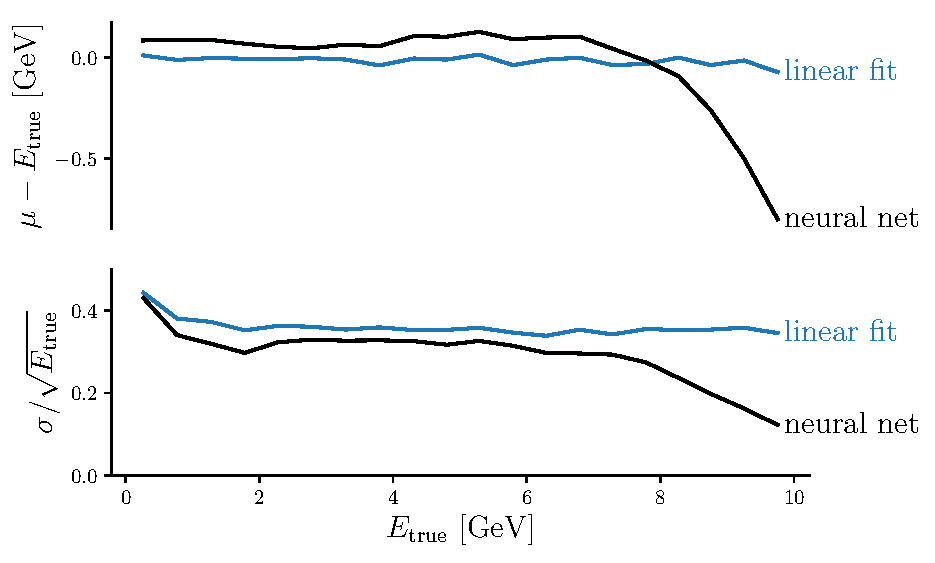
\includegraphics[width=1.1\textwidth]{../data_augment_res.pdf}
    \end{figure}
  \end{columns}
\end{frame}

\begin{frame}{Maximum Likelihood Loss}
Assumption: true values are gaussian distributed with const std $\sigma$
  \begin{align*}
    \text{max likelihood} &= \text{max} \prod \frac{1}{\sqrt{2\pi \sigma^2}} e^{-\frac{(y_{\text{true}}-y_{\text{pred}})^2}{2 \sigma^2}}                          \\
    \Rightarrow \text{max log likelihood} & =\text{max} \sum -\frac{(y_{\text{true}}-y_{\text{pred}})^2}{2 \sigma^2} - \ln(\sqrt{2\pi \sigma^2})                  \\
                                          & =-\text{max} \sum\frac{(y_{\text{true}}-y_{\text{pred}})^2}{\cancel{2 \sigma^2}} - \cancel{\ln(\sqrt{2\pi \sigma^2})} \\
                                          & = \text{min} \sum (y_{\text{true}}-y_{\text{pred}})^2
  \end{align*}
\end{frame}

\begin{frame}{Maximum Likelihood Loss}
  \begin{textblock*}{150pt}(30pt,35pt)
      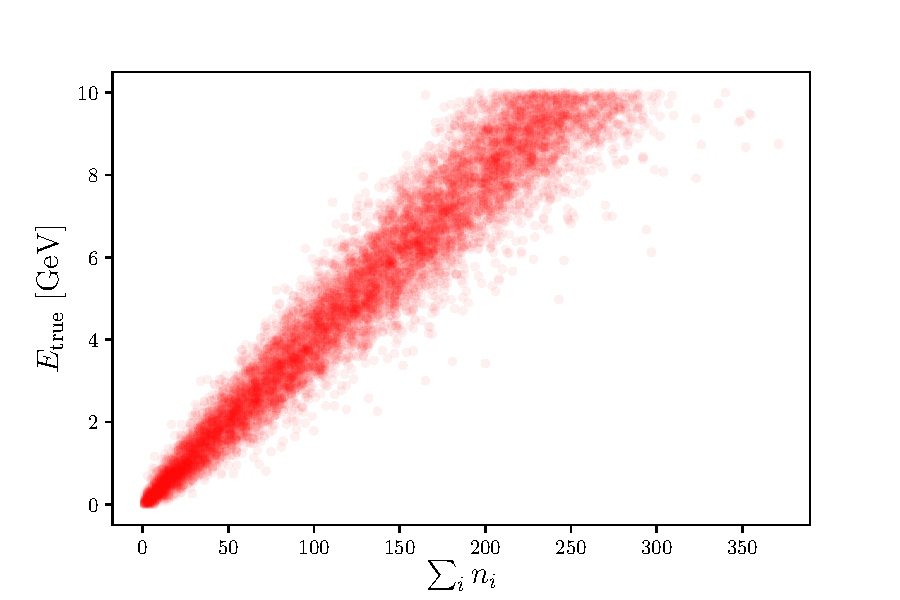
\includegraphics[width=\textwidth]{../e-vs-sum_n.pdf}
  \end{textblock*}
  \begin{textblock*}{150pt}(175pt,35pt)
    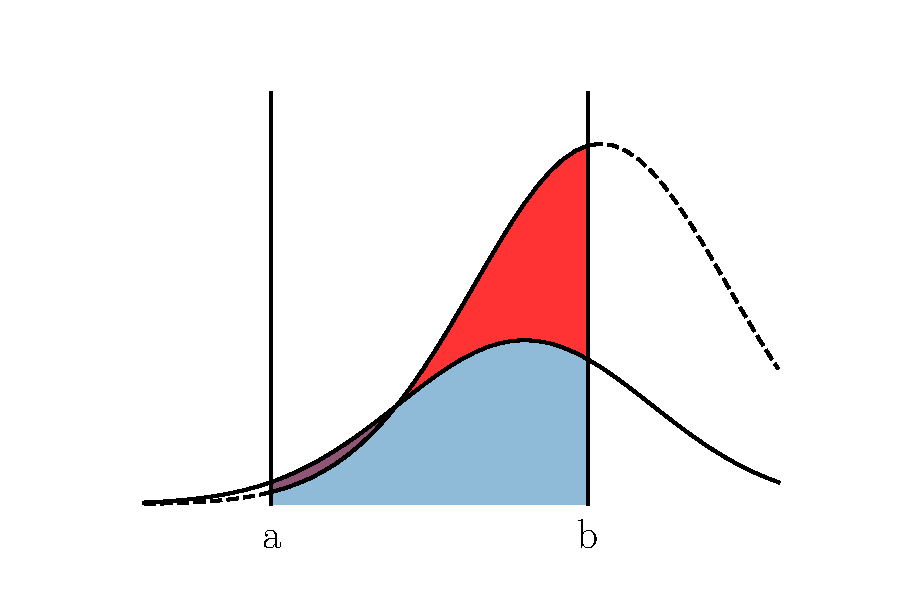
\includegraphics[width=\textwidth]{./gaussian_shift.pdf}
  \end{textblock*}

  \begin{textblock*}{150pt}(5pt,140pt)
    \begin{align*}
      \Rightarrow \text{max log likelihood} = \text{min} \sum& \ln(\frac{\text{Norm}(y_{\text{true}} | y_{\text{pred}}, \sigma)}{\int^b_a \text{Norm}(y_{\text{true}} | y_{\text{pred}}, \sigma)})\\
                                            =\text{min} \sum& \frac{(y_{\text{true}}-y_{\text{pred}})^2}{2 \sigma^2}\\
   &+\ln(\frac{1}{2} \left(\text{erf}(\frac{y_{\text{pred}}-a}{\sqrt{2}\sigma}) - \text{erf}(\frac{y_{\text{pred}}-b}{\sqrt{2}\sigma})\right))
    \end{align*}
  \end{textblock*}
\end{frame}

\begin{frame}{Maximum Likelihood Loss}
  \begin{textblock*}{150pt}(150pt,55pt)
    $\sigma = 0.31 \sqrt{y_{\text{true}}}$
  \end{textblock*}
  \begin{columns}
    \column{0.5\textwidth}
    \begin{figure}[htp]
      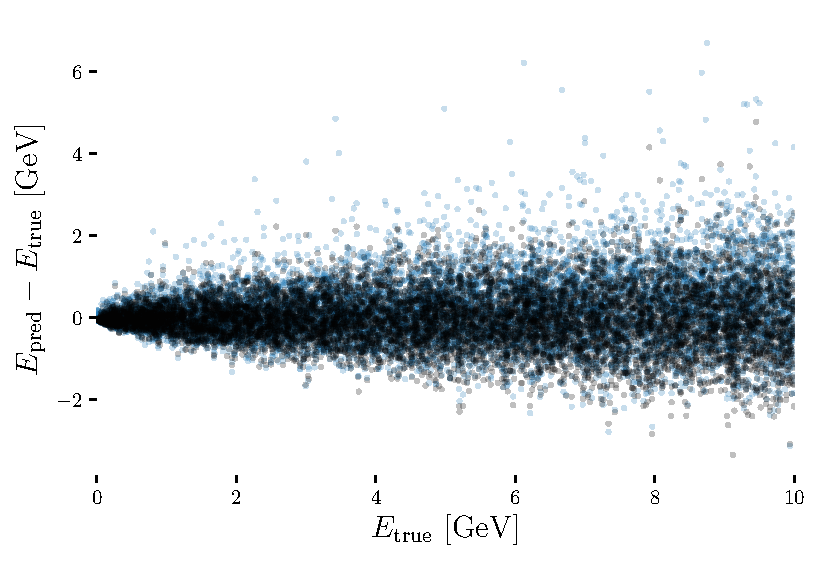
\includegraphics[width=1.1\textwidth]{../likelihood.pdf}
    \end{figure}
    \column{0.5\textwidth}
    \begin{figure}[htp]
      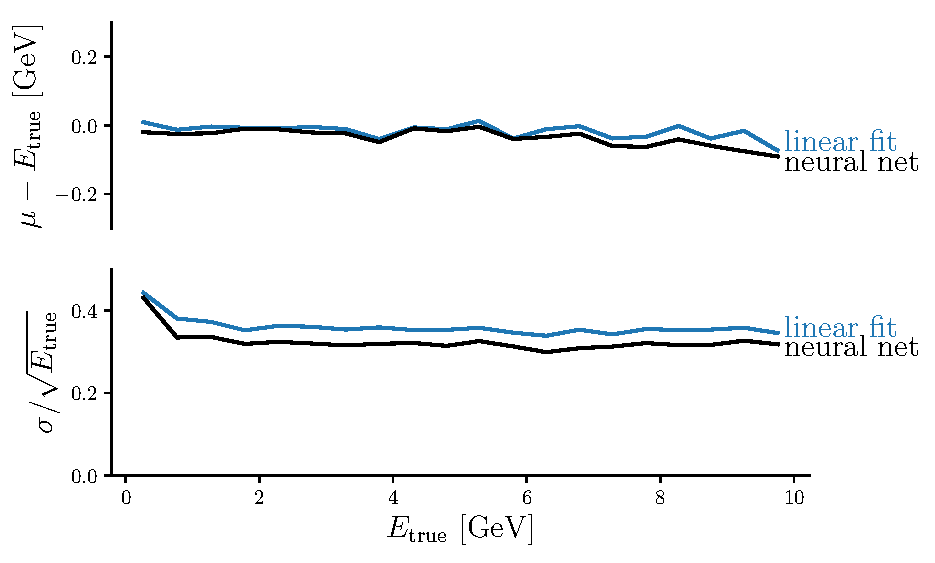
\includegraphics[width=1.1\textwidth]{../likelihood_res.pdf}
    \end{figure}
  \end{columns}
\end{frame}

\begin{frame}{Adversarial Training}

\end{frame}

\begin{frame}{Adversarial Training}
  \begin{columns}
    \column{0.5\textwidth}
    \begin{figure}[htp]
      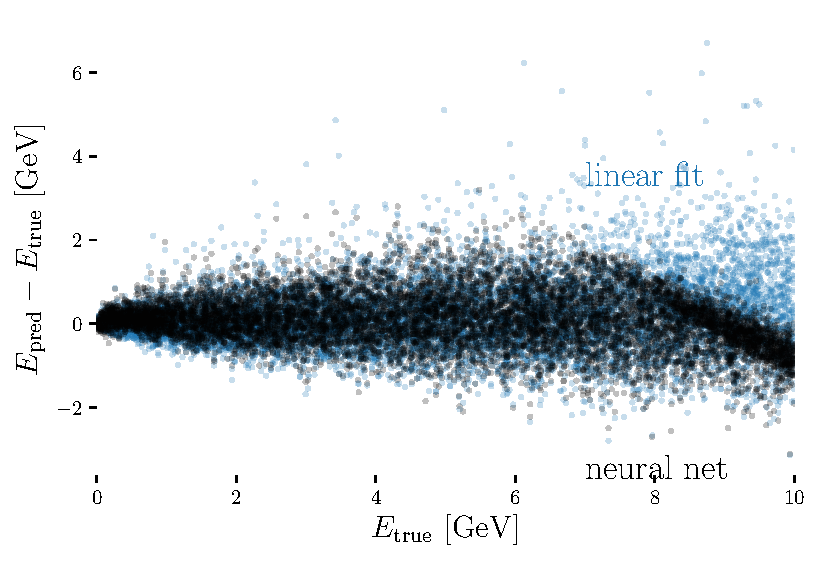
\includegraphics[width=1.1\textwidth]{../adversarial.pdf}
    \end{figure}
    \column{0.5\textwidth}
    \begin{figure}[htp]
      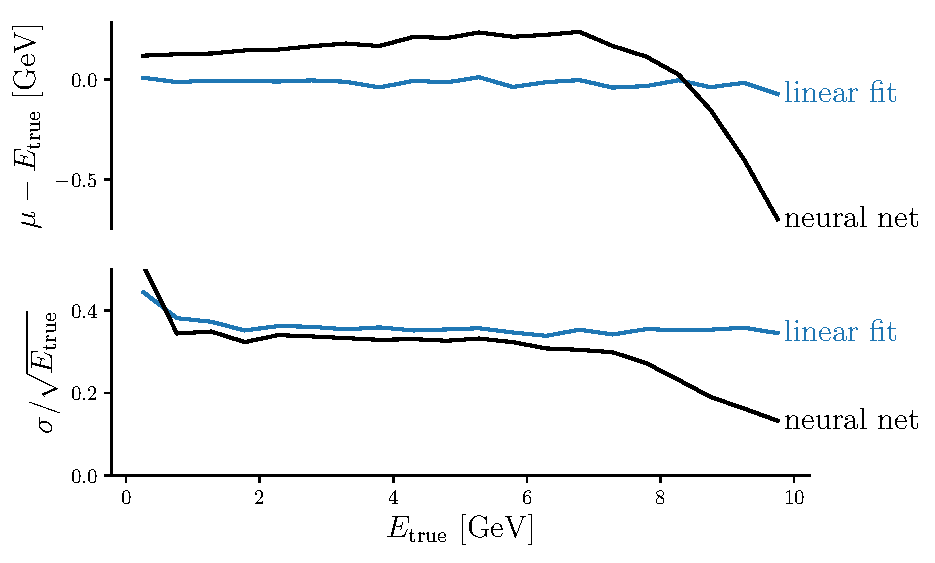
\includegraphics[width=1.1\textwidth]{../adversarial_res.pdf}
    \end{figure}
  \end{columns}
\end{frame}

\begin{frame}{Summary}

\end{frame}

\end{document}
